\documentclass[11pt, twoside]{article} %iniciación del documento de tipo artículo, con tamaño de letra 11pt.
\usepackage[a4paper,total={6in, 8in},left=25mm, asymmetric]{geometry} %Cambio en los bordes y margenes del documento

\usepackage{fancyhdr} %Paquete para organizar y añadir header con los nombres

\usepackage{amsmath}

\usepackage[spanish,es-tabla,es-nodecimaldot]{babel}
\usepackage{tabularx}
\usepackage{booktabs}

\usepackage{caption}
\usepackage{subcaption}

\usepackage{graphicx}
\usepackage[hidelinks]{hyperref}
\usepackage{macro}

\fancypagestyle{main}{
    \fancyhf{}
    \fancyhead[L]{\thepage}
    \fancyhead[RO]{Z. Liu}
    \renewcommand{\headrulewidth}{.4pt}
    \setlength{\headheight}{52pt}
}

\pagestyle{empty}

\begin{document}

\begin{figure}[h!]
    \minipage{0.87\textwidth}
	
\includegraphics[width=3cm]{Icons/ugr.jpg}
	\endminipage
    \minipage{0.87\textwidth}
	
\includegraphics[height = 2.5cm, width=3cm]{Icons/facultad_ciencias.png}
	\endminipage
	%%\vspace{-1cm}
\end{figure}

\vspace{0.3cm}

\begin{center}
    \Huge \textbf{Física Computacional}\\
    		\vspace{0.4cm}
    \LARGE \textbf{Voluntario 2:}  
    Estudio del péndulo doble con un algoritmo Runge-Kutta.
\end{center}

\vspace{1cm}

\vspace{1cm}

\begin{center}
    \large \textbf{Resumen}\\
    		\vspace{0.2cm}
    \normalsize
    En este informe tenemos como objetivo estudiar el comportamiento del 
    doble pendulo, empleando el método de Runge-Kutta para simular el
    movimiento del sistema. Se estudiará la relación entre sus variables
    y la energía total del sistema, para distintas condiciones iniciales.
    Además se analizará la estabilidad del sistema, la influencia pequeñas 
    perturbaciones y la optimización del código.

\end{center}

\vspace{1cm}

\begin{flushright}
    \large ZhuoZhuo Liu 
    \\
    \vspace{0.4cm}
    \textbf{Grado en Física}
\end{flushright}

\newpage

\setcounter{page}{0}
\tableofcontents
\newpage

\pagestyle{main}

\section{Introducción}

\section{Planteamiento del problema}
\subsection{Ecuaciones del movimiento}
Primero debemos de hallar las expresiones de los momentos angulares
a partir del Lagrangiano del sistema. 

\begin{equation}
    \mathcal{L} = \dot{\phi}^2 + \dot{\phi}\dot{\psi} \cos(\psi - \phi) +
     \frac{1}{2}\dot{\psi}^2 - 2g(1-\cos\phi) - g(1-\cos\psi) 
\end{equation}

Hallamos las expresiones del momento angular $p_\phi$ y $p_\psi$, en función
de las velocidades angulares $\dot{\phi}$ y $\dot{\psi}$ através de las 
parciales de $\mathcal{L}$ con respecto a las velocidades angulares.

\begin{equation}
    p_\phi = \frac{\partial \mathcal{L}}{\partial \dot{\phi}} = 2\dot{\phi} + \dot{\psi}\cos(\psi - \phi)
\end{equation}

\begin{equation}
    p_\psi = \frac{\partial \mathcal{L}}{\partial \dot{\psi}} = \dot{\psi} + \dot{\phi}\cos(\psi - \phi)
\end{equation}

Despejando las velocidades en función del momento, permite expresar el 
Hamiltoniano en función de dichos momentos.

\begin{equation}
    \dot{\phi} = \frac{p_\phi - p_\psi\cos(\psi - \phi)}{2-\cos^2(\psi - \phi)}, \quad 
    \dot{\psi} = \frac{2p_\psi - p_\phi\cos(\psi - \phi)}{2-\cos^2(\psi - \phi)}
\end{equation}

\begin{equation}
    \begin{split}
        H &= \dot{\phi}^2 + \dot{\phi}\dot{\psi} \cos(\psi - \phi) +
\frac{1}{2}\dot{\psi}^2 + 2g(1-\cos\phi) + g(1-\cos\psi)  \\
 &=\frac{p_\phi^2 + p_\psi^2 - 2p_\phi p_\psi \cos(\psi - \phi)}{2-\cos^2(\psi - \phi)} + 2g(1-\cos\phi) + g(1-\cos\psi)
    \end{split}
\end{equation}

De donde se obtiene las ecuaciones de movimiento a partir de las 
ecuaciones de Hamilton.

\begin{equation}
        \dot{\phi} = \frac{\partial H}{\partial p_\phi} = \frac{p_\phi - p_\psi\cos(\psi - \phi)}{2-\cos^2(\psi - \phi)} 
\end{equation}

\begin{equation}
    \dot{\psi} = \frac{\partial H}{\partial p_\psi} = \frac{2p_\psi - p_\phi\cos(\psi - \phi)}{2-\cos^2(\psi - \phi)}
\end{equation}

\begin{equation}
    \dot{p_\phi} = -\frac{\partial H}{\partial \phi} =  \frac{p_\phi p_\psi \cos^2(\psi - \phi) - (2p_\psi^2 + p_\phi^2)\cos(\psi - \phi) + 2p_\phi p_\psi }{(2-\cos^2(\psi - \phi))^2}2\sin(\phi - \psi) -2g\sin\phi
\end{equation}

\begin{equation}
    \dot{p_\psi} = -\frac{\partial H}{\partial \psi} =  \frac{p_\phi p_\psi \cos^2(\psi - \phi) - (2p_\psi^2 + p_\phi^2)\cos(\psi - \phi) + 2p_\phi p_\psi }{(2-\cos^2(\psi - \phi))^2}2\sin(\psi - \phi) -g\sin\psi
\end{equation}

\subsection{Condiciones iniciales}

Para este tipos de sistemas, las condiciones iniciales son de suma 
importancia para los resultados obtenidos. Tendremos 3 parámetros que tomar
en cuenta, la energía total del sistema y la ángulo inicial de $\phi$ y
$\psi$, ya que se ha considerado $\dot{\psi} (t=0) = 0$ para simplificar.

Depediendo el objetivo del apartado, se irá variando la energía total 
del sistema, los ángulos iniciales, o ambos. Pero es importante tener en
cuenta que la energía total del sistema no puede ser negativa, ya que
la energía potencial es siempre positiva, esto produce ángulos iniciales
incompatibles con la energía propuesta. De modo que para los estudios donde
se varíe la energía, emplearemos ángulos iniciales relativamente pequeños, 
para que sea compatible con la menor energía propuesta.

\subsection{Unidades empleadas}

Aunque se podría realizar en unidades arbitrarias, en el análisis 
de los resultados se asumirá que todos los valores mensionados se 
encuentran en el sistema internacional. Se debe de tomar en cuenta que 
en el hamiltoniano no aparece ni la masa ni la longitud de los hilos 
ya que se han considerado que son iguales con valor 1, es decir 1 kg y 
1 m respectivamente. 

Tambien se ha considerado la gravedad terrestre, de modo que 
$g = 9.81 \text{m/s}^2$. Y para el resto de variables tendrán las 
siguientes unidades:

\begin{itemize}
    \item $\phi$ y $\psi$ en radianes.
    \item $p_\phi$ y $p_\psi$ en $[\text{kg m}^2/\text{s}]$.
    \item $E$ en $[\text{kg m}^2/\text{s}^2]$, es decir en julios [J].
\end{itemize}


\newpage
\section{Análisis de resultados}

\subsection{Mapas de Poincaré}

Para estudiar el movimiento del sistema, emplearemos los mapas de 
Poincaré para visualizar la relación entre las variables del sistema. 
Comenzando con la relación entre $\phi$ y $\psi$, para distintas 
energías (E = 1, 3, 5, 10, 15). Obteniendo la figura 
\ref{fig:poincare_energias}.

Se aprecia como los ángulos en este caso no superan a $\pi$, de modo
con estas condiciones iniciales, el pendulo no da vueltas completas, 
y esto se ve reflejado en el mapa de Poincaré. 
\begin{figure}[h!]
    \centering
    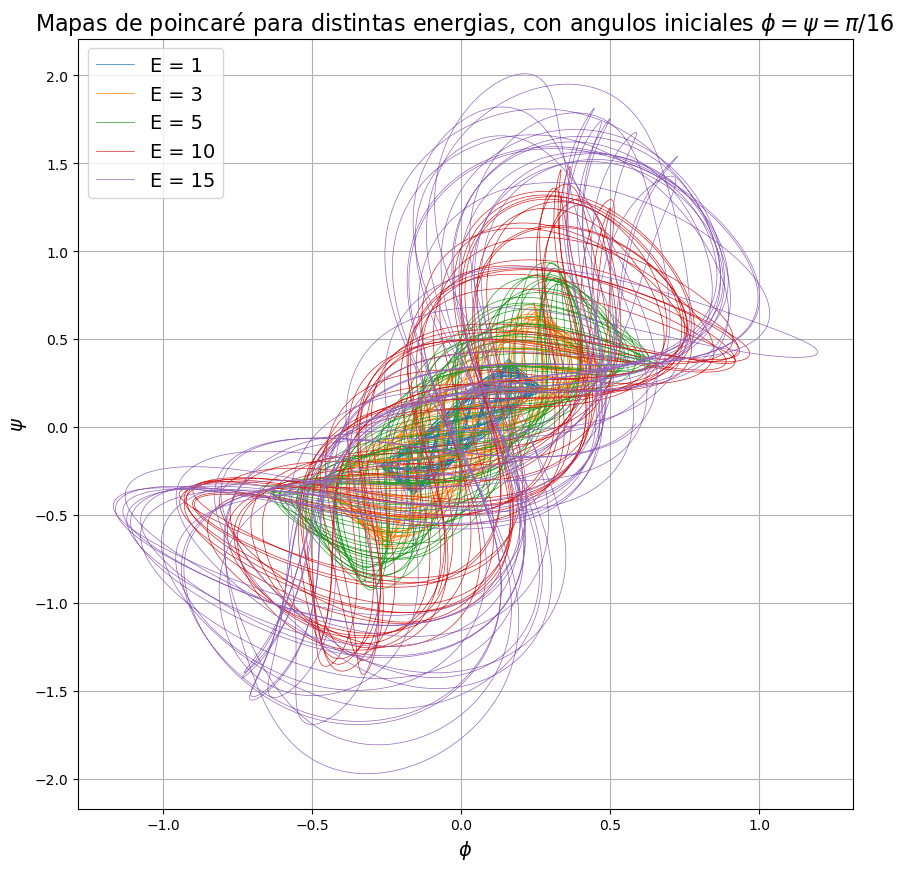
\includegraphics[width=0.9\textwidth]{plots/poincare_energias.png}
    \caption{Mapa de Poincaré para distintas energías}
    \label{fig:poincare_energias}
\end{figure}

Centrandonos en el caso donde la energía $E = 1$ 
(figura \ref{fig:poincare_energia_1}) se puede observar que el sistema 
tiende a ciertas configuraciones, es decir que ciertas combinaciones de 
ángulos $\phi$ y $\psi$ se repiten. Estas combinaciones de estados son 
los atractores del sistema.

\begin{figure}[h!]
    \centering
    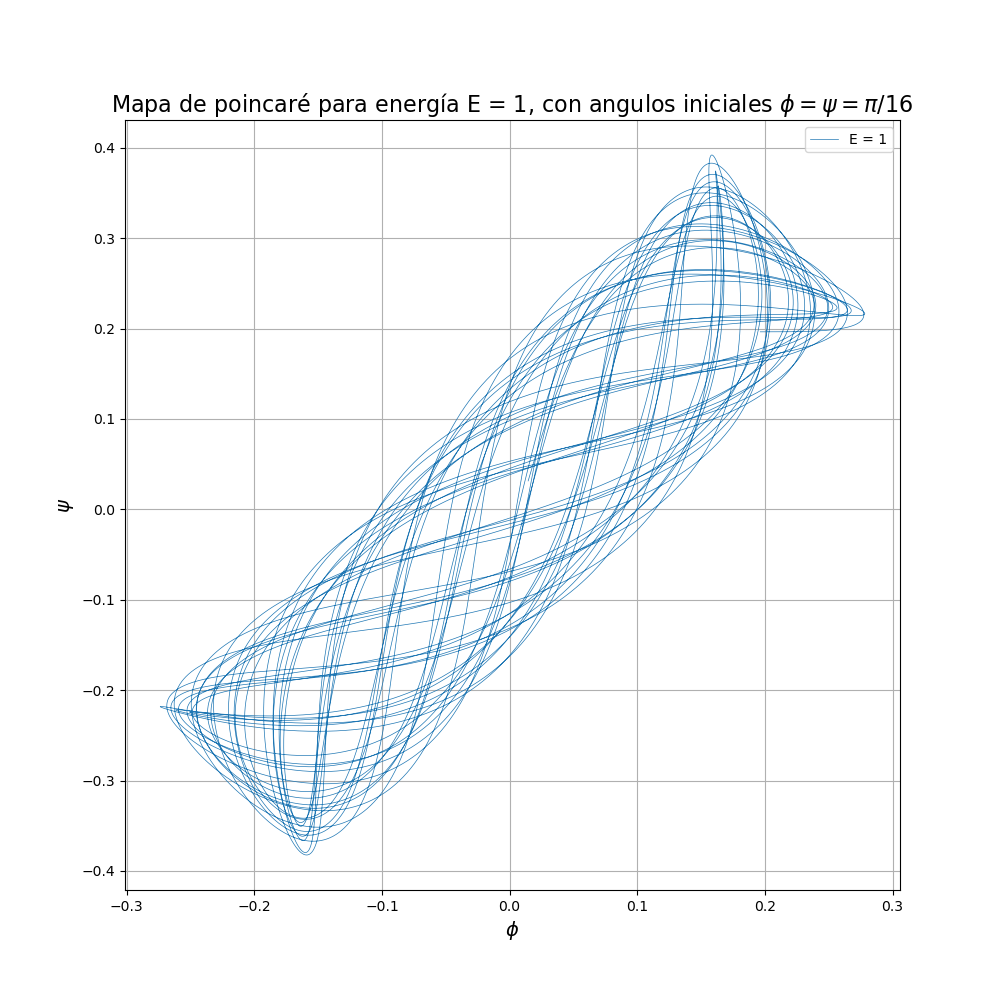
\includegraphics[width=0.9\textwidth]{plots/poincare_energias_1.png}
    \caption{Mapa de Poincaré para E = 1}
    \label{fig:poincare_energia_1}
\end{figure}

Para energías mayores, se va deformando la forma inicial, alcanzando a 
ángulos superiores, pero se sigue observando la misma tendencia a ciertas 
combinaciones de ángulos, solapando ciertas combinaciones, para energías
adjascentes.

Representado los ángulos con sus velocidades angulares, se obtienen otros 
mapas de poincaré (figura \ref{fig:poincare_energias_phi_psi}). En este caso
se observan trayectorias con forma de espiral, esto se debe a la relación entre
dichas variables. También se sigue observando repeticiones en las combinaciones
de ángulos, es decir los atractores del sistema.

Intuitivamente se requiere una velocidad mayor para alcanzar ángulos mayores,
es decir una energía cinética mayor, para alcanzar energías potenciales mayores. 
No es posible tratar los 2 ángulos por separado, ya que el sistema está acoplado, 
sin embargo plantar la conservación de la energía bajo estas condiciones 
puede ser útil para comprender el por qué de las formas circulares en el mapa de
poincaré. Por otro lado el cambio en la amplitud de las espirales, se debe al 
intercambio de energía entre los dos grados de libertad.

\begin{figure}[h!]
    \centering
    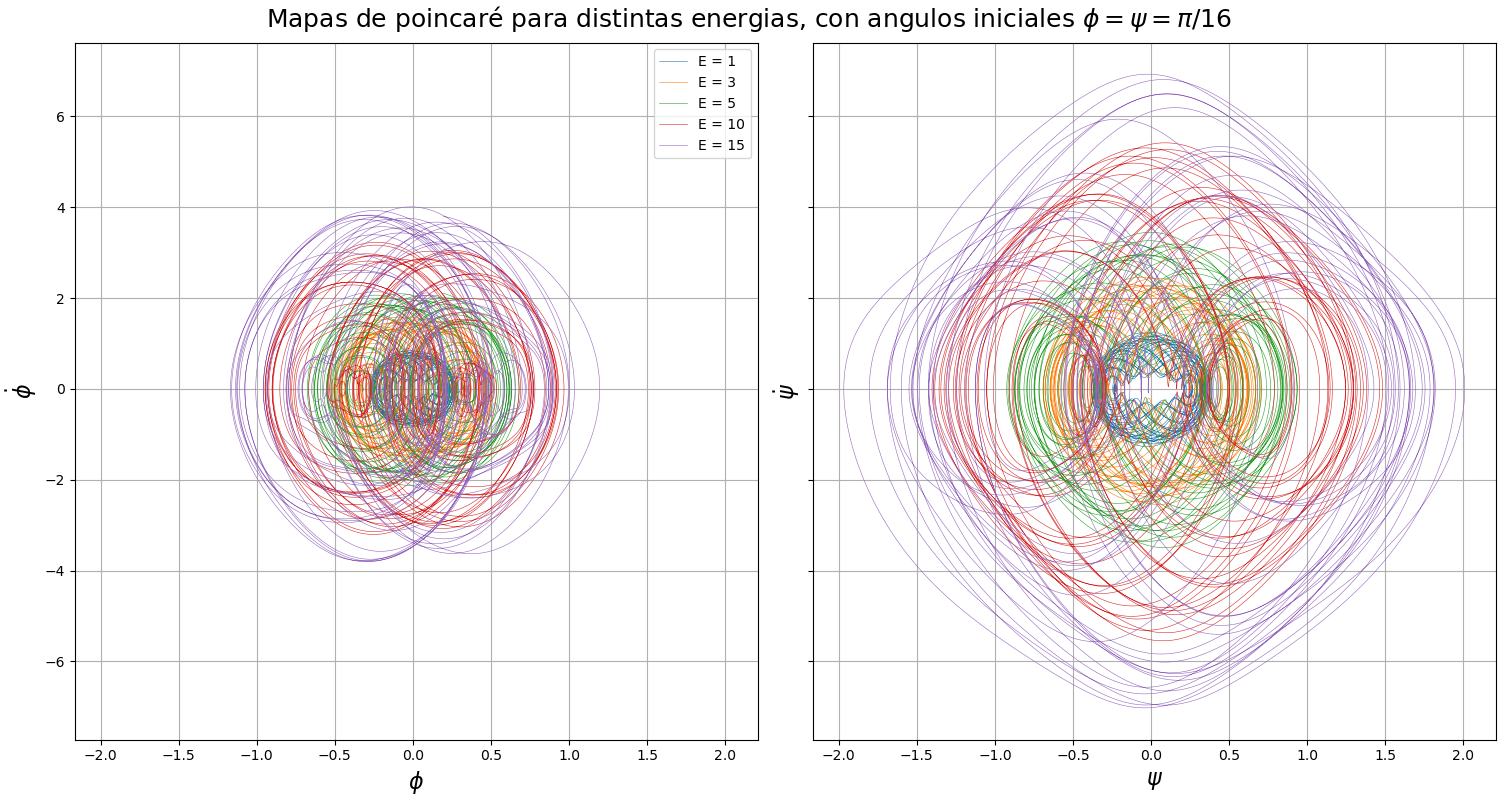
\includegraphics[width=\textwidth]{plots/poincare_energias_phi_psi.png}
    \caption{Mapa de poincaré mostrando la relación entre $\phi$ y $\dot{\phi}$, 
    así como $\psi$ y $\dot{\psi}$, para distintas energías.}
    \label{fig:poincare_energias_phi_psi}
\end{figure}

Cabe notar que la figura para $\psi$ y $\dot{\psi}$ tiene dimensiones 
aproximadamente el doble que la de $\phi$ y $\dot{\phi}$, esto se debe a
la facilidad que tiene el sistema aumentar el ángulo en $\psi$, comparado 
con $\phi$, ya que requiere el movimiento de una única masa, frente a las 2.

\subsection{Coeficiente de Lyapunov}

Para un sistema caótico, el coeficiente de Lyapunov nos permite
cuantificar la tasa de divergencia de dos trayectorias infinitamente
cercanas. Como no es posible tener una separación inicial infinitamente
cercana en la práctica, se tomará un número muy pequeño tal que los
resultados no sean truncados por la máquina

Considerando una separación inicial $\delta \psi_0 = 10^{-15}$, 
al cabo de un tiempo $t$, la separación entre las dos trayectorias será 
$\delta \psi (t)$, la relación entre ambas viene dado por:
\begin{equation}
    |\delta \psi (t)| \approx |\delta \psi_0| e^{\lambda t}, 
\end{equation}
con $\lambda$ el coeficiente de Lyapunov.

Tomando la evolución de fracción de la separación a tiempo $t$ respecto 
a la inicial, se obtiene la figura, donde se realiza un ajuste exponencial
para obtener el coeficiente de Lyapunov.

\begin{figure}
    \begin{subfigure}{.5\textwidth}
      \centering
      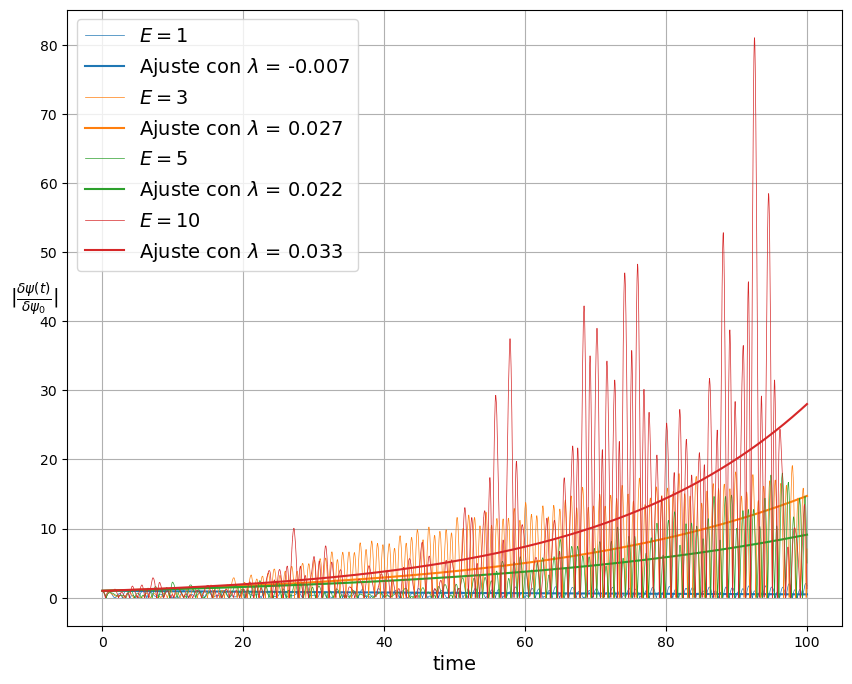
\includegraphics[width=\linewidth]{plots/coeficientes_lyapunov_1_4.png}
      \label{fig:coeficiente_lyapunov_1_4}
    \end{subfigure}%
    \begin{subfigure}{.5\textwidth}
      \centering
      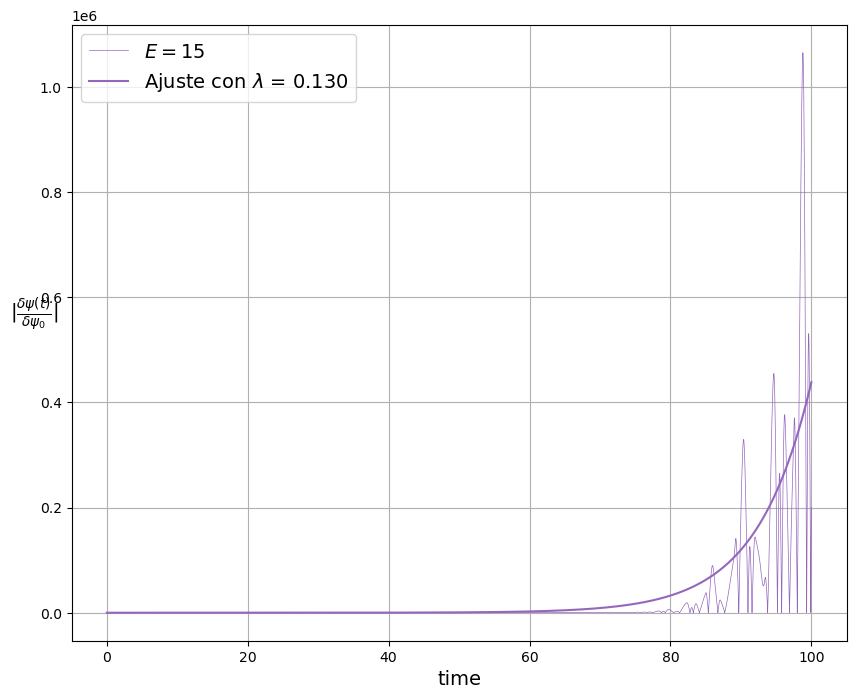
\includegraphics[width=\linewidth]{plots/coeficientes_lyapunov_5.png}
      \label{fig:coeficiente_lyapunov_5}
    \end{subfigure}
    \caption{plots of....}
    \label{fig:coeficiente_lyapunov}
\end{figure}

En la figura \ref{fig:coeficiente_lyapunov} se observa como el coeficiente
de Lyapunov aumenta con la energía del sistema, esto indica que el sistema
es más caótico a medida que aumenta la energía.

\subsection{Estabilidad del sistema}

Para estudiar la estabilidad del sistema, se ha considerado pequeñas
variaciones en las condiciones iniciales, a diferentes valores de 
energía. Emplearemos nuevamente los mapas de poincaré, determinado que 
un sistema es estable si las variaciones iniciales no afectan en gran medida
la forma que tiene los mapas de poincaré.

Comenzando con las variaciones en la energía del sistema, para ángulos 
iniciales bajos, para poder emplear los mismos ángulos iniciales para los 
distintos casos, siendo estas $\phi_0 = \psi_0 = \pi/16$, se irá viendo como 
afecta la perturbación del ángulo $\psi_0$ a la evolución del sistema.

\begin{figure}
    \begin{subfigure}{.5\textwidth}
      \centering
      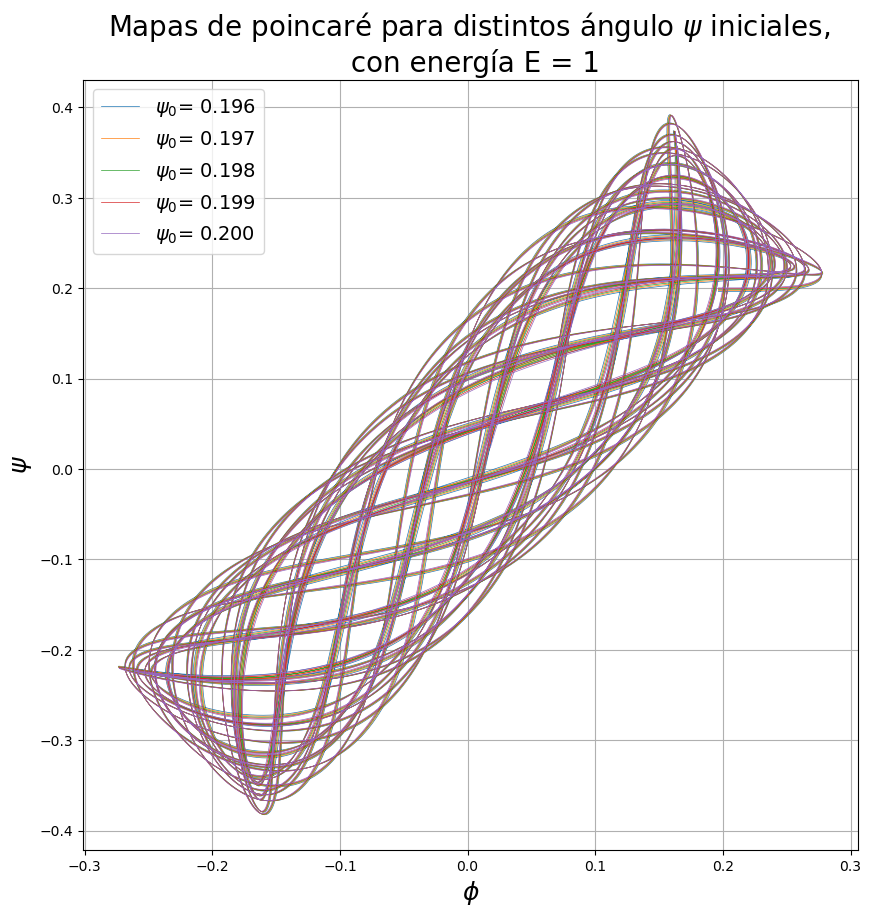
\includegraphics[width=\linewidth]{plots/poincare_estabilidad_E_1.png}
      \label{fig:poincare_estabilidad_E_1}
    \end{subfigure}%
    \begin{subfigure}{.5\textwidth}
      \centering
      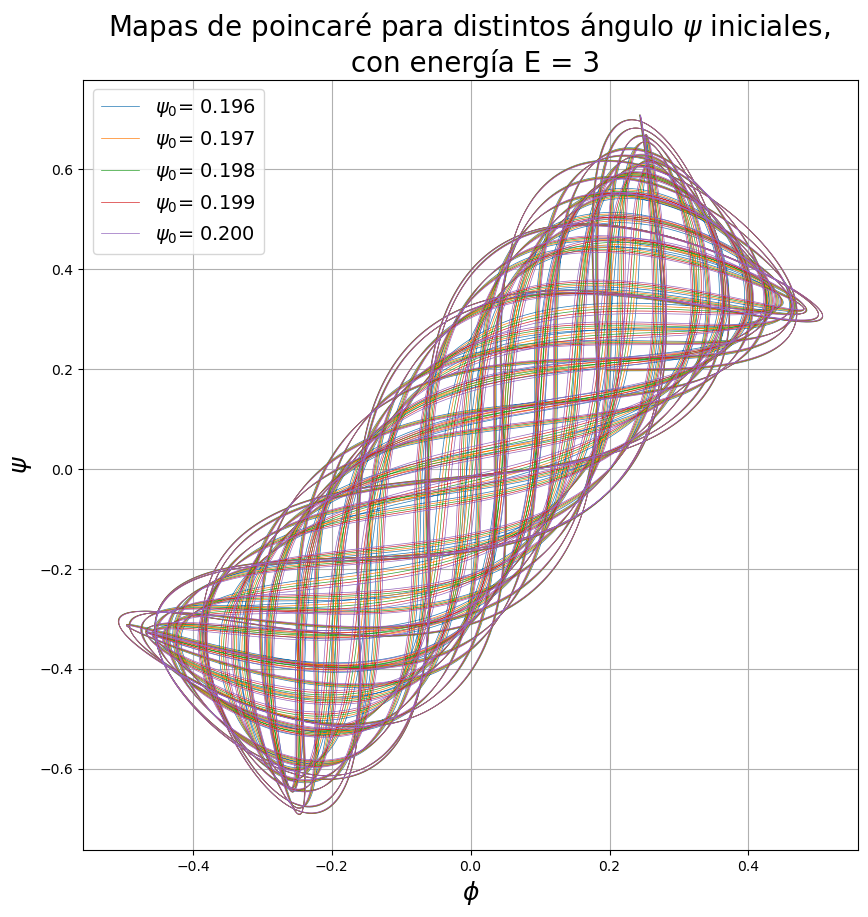
\includegraphics[width=\linewidth]{plots/poincare_estabilidad_E_3.png}
      \label{fig:poincare_estabilidad_E_3}
    \end{subfigure}
    \begin{subfigure}{.5\textwidth}
        \centering
        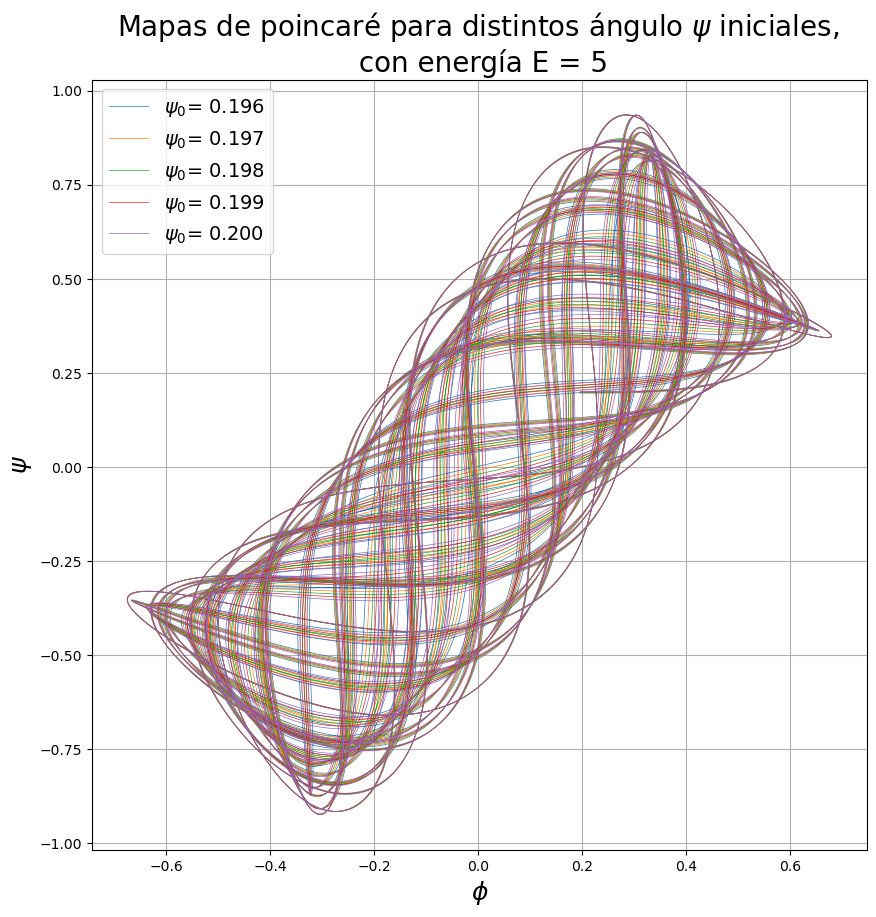
\includegraphics[width=\linewidth]{plots/poincare_estabilidad_E_5.png}
        \label{fig:poincare_estabilidad_E_5}
      \end{subfigure}%
      \begin{subfigure}{.5\textwidth}
        \centering
        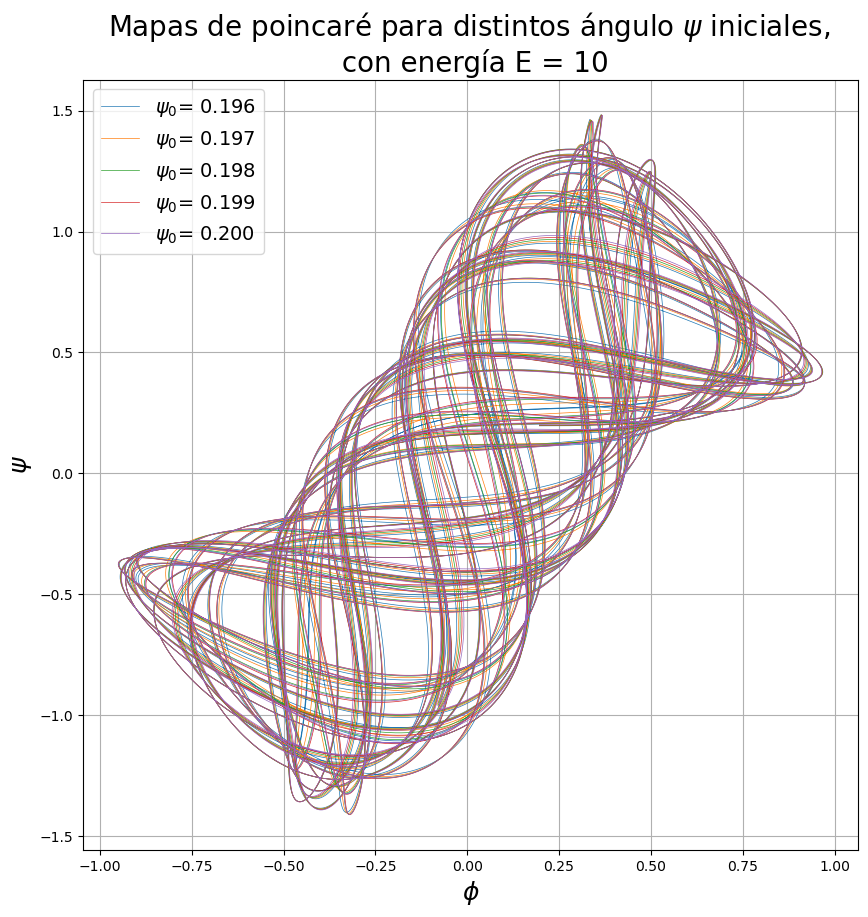
\includegraphics[width=\linewidth]{plots/poincare_estabilidad_E_10.png}
        \label{fig:poincare_estabilidad_E_10}
      \end{subfigure}
    \caption{plots of....}
    \label{fig:poincare_estabilidad_E}
\end{figure}
    
\begin{figure}[h!]
    \centering
    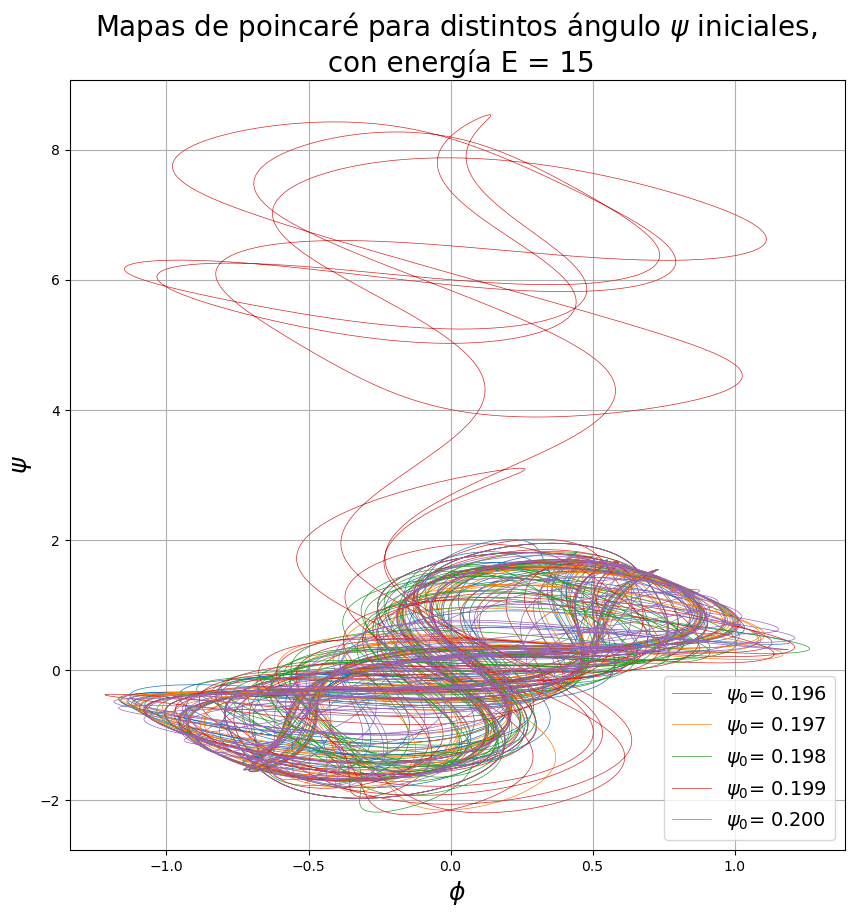
\includegraphics[width=0.75\linewidth]{plots/poincare_estabilidad_E_15.png}
    \caption{plots of....}
    \label{fig:poincare_estabilidad_E_15}
\end{figure}

En las figuras \ref{fig:poincare_estabilidad_E} y \ref{fig:poincare_estabilidad_E_15} 
se observa como la perturbación en el ángulo $\psi_0$ afecta a la evolución 
del sistema para distintos niveles de energía. En concreto se observa como 
a niveles de energías bajos, los mapas de poincaré apenas varían entre las
diferentes configuraciones iniciales, sin embargo a medida que aumenta la
energia, la perturbación en el ángulo $\psi_0$ afecta en mayor medida a la
evolución del sistema, separando las trayectorias en el mapa de poincaré. 
Esto culmina en el caso de $E = 15$, donde hay un cambio drástico en un ángulo
entre media de otros, lo que indica que el sistema es inestable para dichas 
energías.

\newpage

\subsection{Optimización}

Se va a comparar el tiempo de ejecución de los métodos de Runge-Kutta, para 
distintas máquinas, distintos tamaños de paso $h$, y distintos tiempos totales
de simulación. Estos 2 últimos parámetros pueden ser unirse en uno solo, 
el número de interacciones, $N = t/h$. Disminuyendo el tamaño de paso, o 
aumentando el tiempo de simulación, tiene el mismo efecto en cuanto al coste
computacional, ya que este es el parámetro empleado en el programa.

En este caso se ha obviado paralelizar el código, ya que se espera resultados similares
a los obtenidos en el voluntario 1: el potencial de Lennard-Jones, donde se observó 
que el tiempo de ejecución aumentaba al paralelizar el código. Como el procedimiento de
este voluntario es similar, no se empleará la paralelización.

Se ha considerado 3 ordenadores distintos, con las siguientes características:
\begin{itemize}
    \item Portatil windows: Intel Core i5-12500H, 16GB RAM, enchufado.
    \item Portatil Macbook Pro M1 (2020), 8GB RAM, desenchufado.
    \item Joel.
\end{itemize}

\begin{figure}[h!]
    \centering
    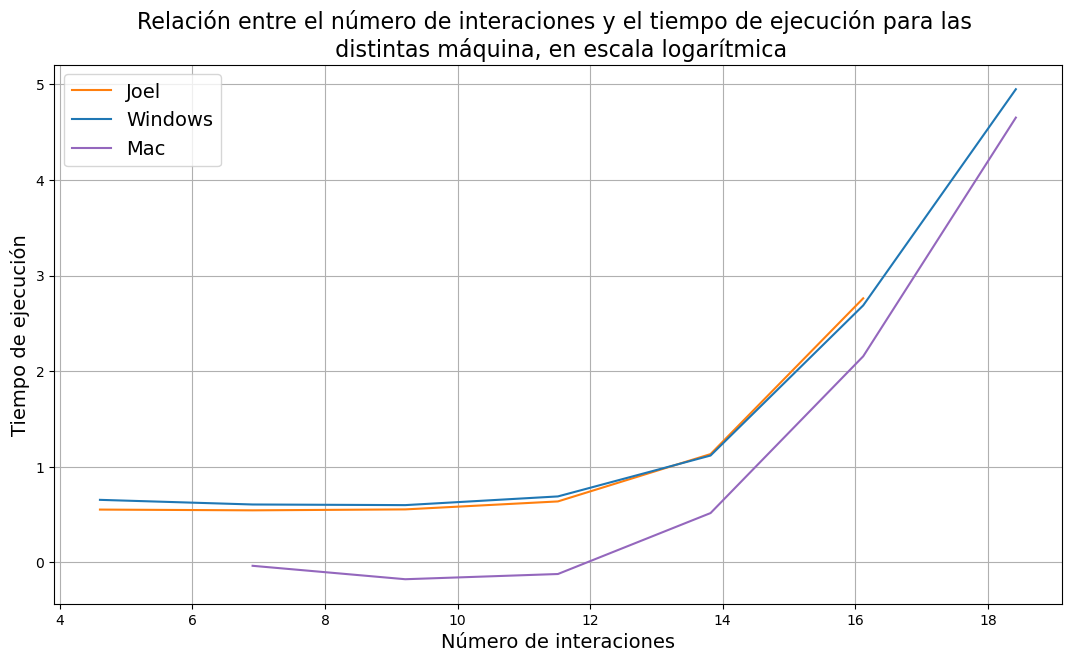
\includegraphics[width=\linewidth]{plots/optimizacion.png}
    \caption{Representación del número de interacciones en relación con el tiempo 
    de ejecución, para las distintas máquinas, en escala logarítimica. Optimizando
    todas las funciones posibles con \texttt{@jit(nopython=True)}.}
    \label{fig:optimizacion}
\end{figure}

Se observa en la figura \ref{fig:optimizacion}, como para Joel, falta el dato 
para número de interacciones de $10^8$, ya que la máquina ha matado el proceso
antes que de pudiera terminar, sin embargo por la forma que tiene la gráfica es 
razonable esperar un comportamiento similar al ordenador de windows.

En cuanto a la forma que tiene el tiempo de ejecución en relación con el número de interacciones esta tiene un comportamiento exponencial.

\newpage

\appendix

\section{Tabla de valores}

Los valores obtenidos en las simulaciones se encuentran en el propio repositorio
donde se puede encontrar también el código empleado para la realización 
de este informe y los gif generados para la visualización de los resultados.

\end{document}
